\chapter[Bugzilla]{Bugzilla \\\small{\textit{-- Charles, Justin, Benedict, Jacky}}}
\label{Chapter::Bugzilla}
\index{Chapter!Bugzilla}

\begin{enumerate}
    \item Setup Cloud Infrastructure and Access
    \begin{itemize}
        \item Created a Digital Ocean account and created a Ubuntu Droplet VM.
        \item Secured access by generating and adding an SSH key to the Droplet.
    \end{itemize}
    
    \item Prepare Container Environment
    \begin{itemize}
        \item Cloned the Bugzilla source code.
        \item Installed and fixed the missing dependencies (Docker Compose and the Docker service daemon) needed to run containers.
    \end{itemize}
    
    \item Deploy Application Containers
    \begin{itemize}
        \item Used Docker Compose to launch two linked services: the Bugzilla web application container and the MariaDB database container.
        \item Ensured the application's internal network port was mapped to the Droplet's external port 8080.
    \end{itemize}
    
    \item Finalize Configuration
    \begin{itemize}
        \item Executed the required Bugzilla setup script (checksetup.pl) inside the running web container to build the database schema and verify system readiness.
    \end{itemize}
    
    \item Access and Admin Creation
    \begin{itemize}
        \item Confirmed the application was accessible in a web browser at the public IP and port (http://174.138.69.132.8080).
        \item Completed the final step by creating the administrator account via the web interface.
        \item Deleted the Droplet (which is why the link might not work anymore) to avoid any unnecessary billing.
    \end{itemize}
    
\end{enumerate}

\begin{figure}[htp]
    \centering
    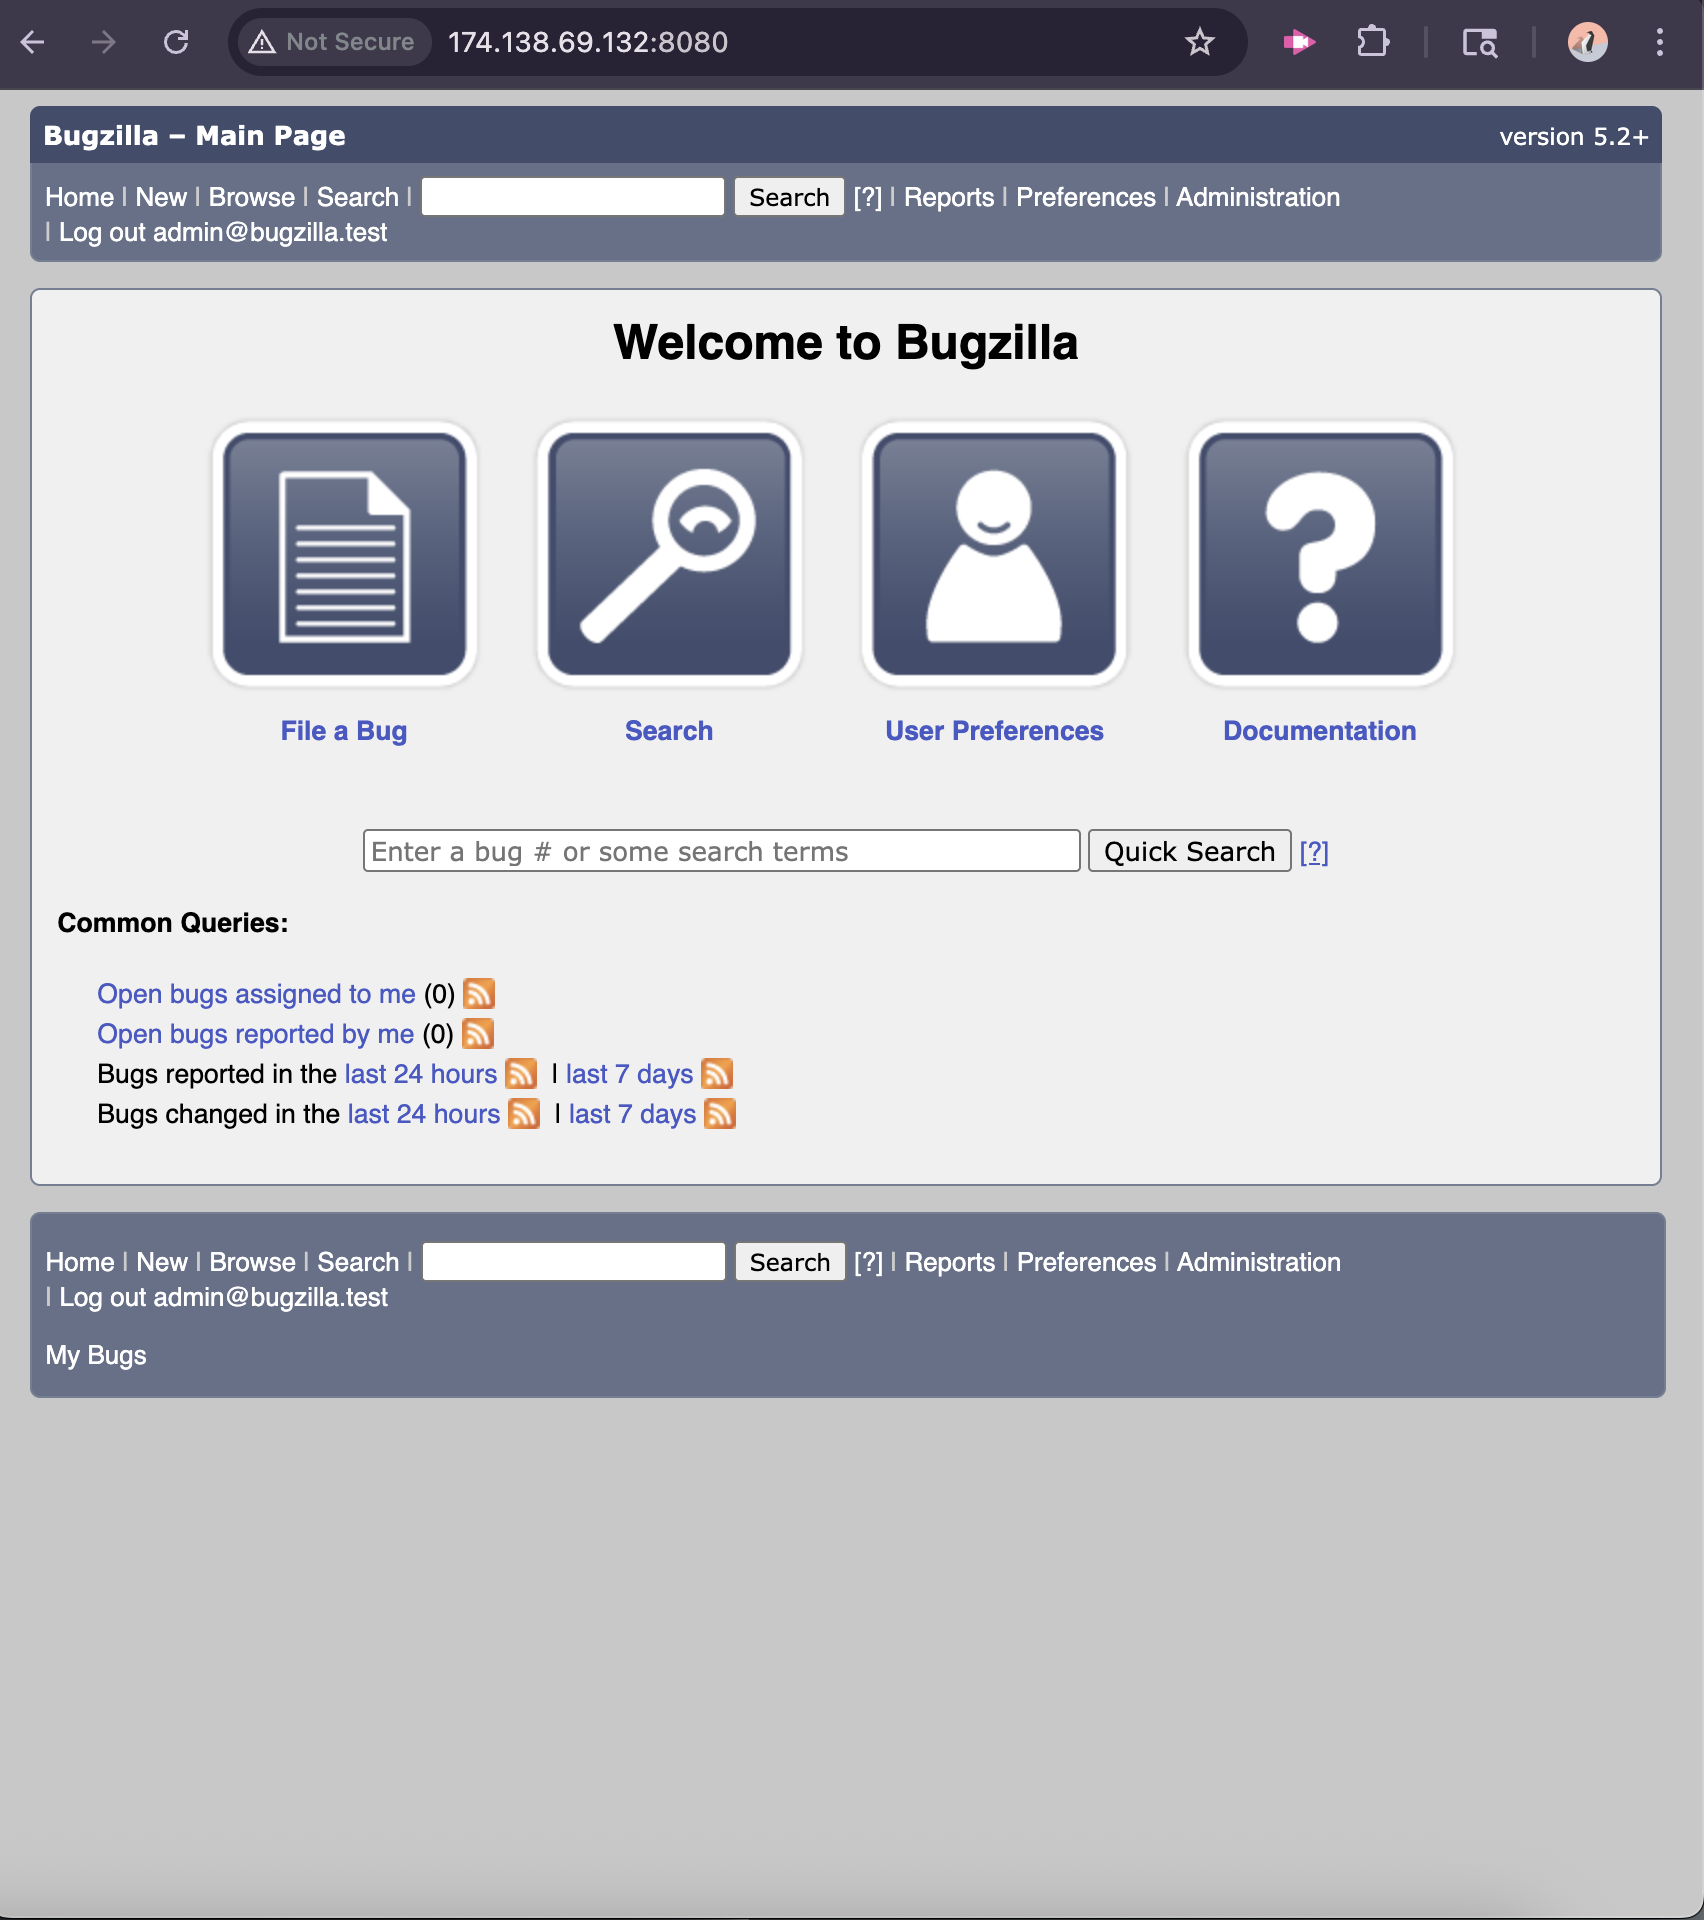
\includegraphics[width=15cm, height=10cm]{png/DigitalOcean/Bugzilla.png}
    \caption{Bugzilla Container Running Screenshot}
    \label{fig:Bugzilla}
\end{figure}